%%%%%%%%%
%
% Trade 
% Notes of research
% Brian Dew
%
%%%%%%%%%
	\documentclass[10pt,letterpaper]{article}

%
% Packages
%
	\usepackage[right=1.6in, left=1.6in, top=1.3in, bottom=1.2in]{geometry}
	\usepackage{pgfplots,pgfplotstable}
	\usepackage{amsmath,amsthm,amssymb}	
	\usepackage{graphicx}
	\usepackage[colorlinks,
  		linkcolor=cyan!50!blue,
  		filecolor=cyan!50!blue,
 		citecolor=cyan!50!blue,
 		urlcolor=cyan!50!blue,
 		linktoc=all]{hyperref}
	\usepackage{calc}
	\usepackage[latin1]{inputenc}
	\usepackage{float}
	\usepackage{array}
	\usepackage{booktabs}
	\usepackage[center]{caption}
	\usepackage{xcolor}
	\usepackage[eulergreek]{sansmath}
	\usepackage{listings}
	\usepackage{parskip}
	\usepackage{bm}
	\usepackage{subcaption}
%
% Title Info
%

	\author{Brian Dew\\ (brian.dew@american.edu)}
	\title{Trade Network Structure and Export Volatility}

\tikzset{
    	every node/.append style={font=\sansmath\sffamily\footnotesize}}

\begin{document}
\maketitle

\section{Theoretical background}
Xavier Gabaix (2011) offered theoretical and empirical evidence against the argument of Lucas (1977) that firm-specific shocks average out. Gabaix showed that 1/3 of output volatility in the United States can be directly tied to changes in the 100 largest U.S. firms. When firm sizes follow a power-law distribution, idiosyncratic shocks do not average out, and actually propagate downstream and affect aggregate economic output. This is because there are often few central suppliers for the key inputs to several industries. A shock to one the central firms causes consequences for all firms that require the input for their own production. I hypothesize that this relationship holds internationally, particularly given actual variation in the volume of exports by product and country, and the rise of international trade of intermediate goods due to global value chains. Equations that seek to attribute local fluctuations in exports to idiosyncratic shocks elsewhere in the world are estimated using two models. 

\section{Theoretical argument}
Three basic points to my argument:

\begin{enumerate}
\item Countries need goods to produce goods (Leontief I-O linkages). Inputs from upstream suppliers are required to produce outputs for downstream consumers.
\item Countries role in the trade of individual goods (specifically their \href{https://en.wikipedia.org/wiki/Centrality}{centrality}) is not uniform, and for some goods, follows a power law distribution\footnote{Defined for this paper as having an estimated alpha value of weighted outdegree centrality scores between 2 and 3, where $p(x) = Cx^{-\alpha}$.}. The extent of this distribution varies from product to product, and can be captured for each product by applying the tools of network analysis.
\item Shocks from upstream are propagated downstream depending on the network structure for the affected product. 
\end{enumerate}

Essentially, this is an argument about how network structure affects whether idiosyncratic shocks propagate or die out. Internationally, does the trade network's tendency to have central exporters affect whether a supply-shock to the imports of an intermediate good are passed-through and reduce exports?

The motivation for this research comes from an anomaly noticed following two recent natural disasters. First, the 2011 Tohoku earthquake and tsunami, which caused massive destruction, loss of life, and a nuclear disaster, also caused supply-shocks in global trade. French automakers were forced to shutter assembly lines after diesel engine imports from Japan were delayed. Likewise, the launch of the iPad 2 was delayed when the Japanese supplier of the cover glass was affected by the disaster. Second, the 2011 Thailand floods disrupted the production of computer hard disk drives, which has been dominated by Thai producers. The price of hard disk drives nearly doubled worldwide and remained elevated for two years. Such disruptions to the supply of key intermediate goods can create a situation where a localized supply-shock (from a natural disaster) results in aggregate fluctuations elsewhere in the world.

\subsubsection*{\centerline{Visual representation: shock to central vs. non-central supplier}}
\vspace{1mm}
\begin{figure}[h]
\caption[]{The effect of a negative shock to Australian iron ore exports depends on network structure. Here circles represent countries, with Australia (AUS) as the localized supply-shock affected country, in orange, countries without a functioning supplier in yellow, and unaffected countries in blue\footnotemark. Solid lines represent unaffected trade flows and dashed lines represent compromised trade flows.} \label{fig:M1}
\centering
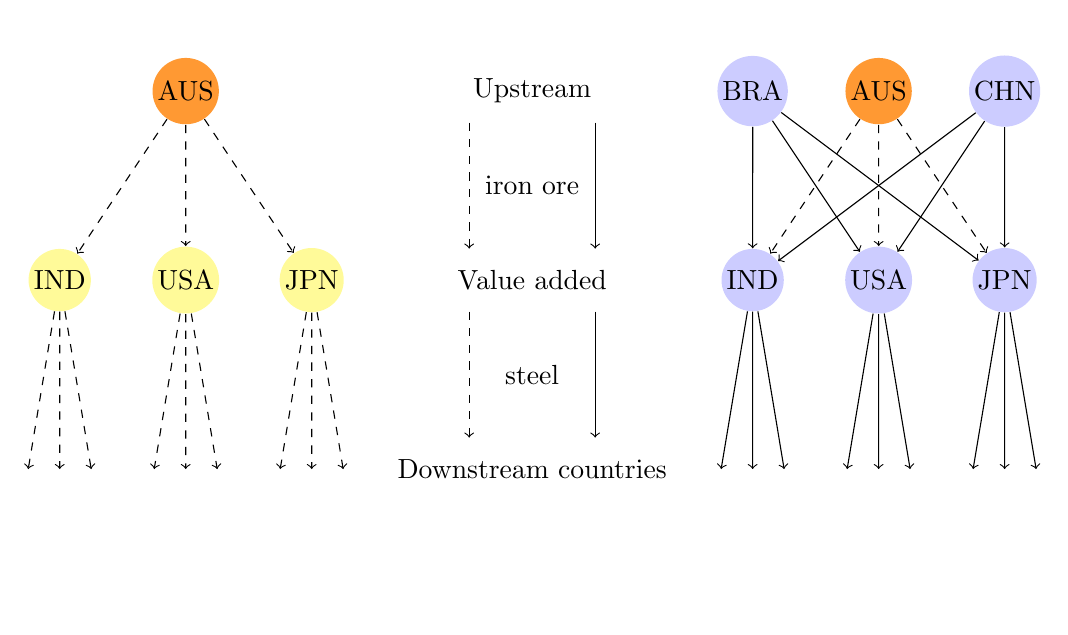
\begin{tikzpicture}
  [scale=.8,auto=left,every node/.style={inner sep=1pt,circle,fill=yellow!40}]
  \node [fill=orange!80] (n6) at (3,10) {AUS};
  \node [draw=none,fill=none] (n7) at (8.5,10) {Upstream};
  \node [draw=none,fill=none] (n8) at (8.5,7) {Value added};
  \node [draw=none,fill=none] (n9) at (8.5,8.5) {iron ore};
  \node [draw=none,fill=none] (n10) at (8.5,4) {Downstream countries};
  \node [draw=none,fill=none] (n11) at (8.5,5.5) {steel};
  \node (n4) at (5,7)  {JPN};
  \node (n5) at (1,7)  {IND};
  \node (n3) at (3,7)  {USA};
  \draw [->, dashed] (7.5,9.5) -- (7.5,7.5);
  \draw [->] (9.5,9.5) -- (9.5,7.5);
  \draw [->, dashed] (7.5,6.5) -- (7.5,4.5);
  \draw [->] (9.5,6.5) -- (9.5,4.5);
  \draw [->, dashed] (n4) -- (5,4);
  \draw [->, dashed] (n4) -- (4.5,4);
  \draw [->, dashed] (n4) -- (5.5,4);
  \draw [->, dashed] (n5) -- (1,4);
  \draw [->, dashed] (n5) -- (0.5,4);
  \draw [->, dashed] (n5) -- (1.5,4);
  \draw [->, dashed] (n3) -- (3,4);
  \draw [->, dashed] (n3) -- (2.5,4);
  \draw [->, dashed] (n3) -- (3.5,4);
  
  \foreach \from/\to in {n6/n4,n6/n5,n6/n3}
    \draw[->, dashed] (\from) -- (\to);
    
  \node [fill=orange!80] (p6) at (14,10) {AUS};
  \node [fill=blue!20] (p2) at (12,10) {BRA};
  \node [fill=blue!20] (p1) at (16,10) {CHN};  
  \node [fill=blue!20] (p4) at (16,7)  {JPN};
  \node [fill=blue!20] (p5) at (12,7)  {IND};
  \node [fill=blue!20] (p3) at (14,7)  {USA};
  \draw [->] (p4) -- (16,4);
  \draw [->] (p4) -- (15.5,4);
  \draw [->] (p4) -- (16.5,4);
  \draw [->] (p5) -- (12,4);
  \draw [->] (p5) -- (11.5,4);
  \draw [->] (p5) -- (12.5,4);
  \draw [->] (p3) -- (14,4);
  \draw [->] (p3) -- (13.5,4);
  \draw [->] (p3) -- (14.5,4);

  \foreach \from/\to in {p2/p3,p2/p4,p2/p5,p1/p5,p1/p3,p1/p4}
    \draw[->] (\from) -- (\to);
    
  \foreach \from/\to in {p6/p4,p6/p5,p6/p3}
 	\draw[->, dashed] (\from) -- (\to);
\end{tikzpicture}
\end{figure}
\footnotetext{There may still be price effects.}
\vspace{-15mm}
\section{Foundations in microeconomics}

The derivation from theory of a testable hypothesis is borrowed almost verbatim from Acemoglu, Akcigit, and Kerr (2016) but adjusted to apply internationally (and to ignore demand shocks) as follows:

We start with a Cobb-Douglas production function for each country:
$$ y_i = e^{z_i}l_i^{\alpha_i^l} \prod_{j=1}^{n} x_{ij}^{a_{ij}}$$

Where $x_{ij}$ is the volume of goods produced by country j and imported to country i, $l_i$ is labor, and $z_i$ is a Hicks-neutral productivity shock. Assume that for each country, $\alpha_i^l >0$, and $a_{ij} \geq 0$ for each pair of countries in the network (if $a_{ij} = 0$, there are no imports to country $i$ from country $j$). Lastly,
$$ \alpha_i^l + \sum_{j=1}^{n} a_{ij} = 1$$

so constant returns to scale are assumed. 

The market clearing condition is:
$$y_i = c_i + \sum_{j=1}^{n} x_{ji}$$

where $c_i$ is domestic consumption and an amount of goods is also exported to each of $n$ countries.

The downward sloping line comes from preferences of a representative household:
$$ u(c_1,c_2,...,c_n,l) = \gamma (l) \prod_{i=1}^{n} c_i^{\beta_i}$$

where $\beta_i$ is distributed between 0 and 1, sums to 1 across all $i$'s, and represents the weight of goods from country $i$ in the representative household's preferences. The disutility of labor is given by the function $\gamma (l)$, which is assumed to be negative.

The household faces the following budget constraint:
$$ \sum_{i=1}^{n} p_ic_i = wl$$

where $w$ is the wage rate, set to 1 for simplicity.

Aggregate profit maximization applied to the Cobb-Douglas production functions determines the individual good trade flows (assuming for simplification that trading costs are CIF and incorporated into $p_j$):
$$ \frac{p_jx_{ij}}{p_iy_i} = a_{ij}$$

Consider therefore an international input-output matrix of $a_{ij}$'s denoted as \textbf{A}:
\begin{equation*}
\text{\textbf{A}} = \begin{bmatrix}
		a_{11} & a_{12} & ... \\
		a_{21} & a_{22} &  \\
		\vdots &  & \ddots 
		\end{bmatrix}
\end{equation*}		

The Leontief inverse of matrix \textbf{A} is defined as:
$$ \mathbf{H} \equiv (\mathbf{I} - \mathbf{A})^{-1} $$

with each entry in matrix \textbf{H} identified as $h_{ij}$.

Acemoglu, Akcigit, and Kerr then propose the following relation for the impact of domestic and foreign shocks on changes to aggregate output:
$$ d \ \text{ln} \ y_i = \underbrace{dz_i}_{\text{own effect}} + \underbrace{\sum_{j=1}^{n} (h_{ij} - \bm{1}_{j=i}) \times dz_j}_{\text{network effect}}$$

where $\bm{1}_{j=i}$ is the indicator function for $j=i$.
\section{Data sources and methods}
The primary data source is the BACI dataset produced by CEPII. BACI provides data on bilateral trade by product at the HS six-digit level of disaggregation. BACI is essentially a cleaned and expanded version of UN Comtrade data. 

Supply-shocks are identified using the EM-DAT database of natural disasters. Such supply shocks are by definition exogenous and location specific. 

Data on total exports, the real effective exchange rate, and import and export prices \footnote{Import and export price indices are used to adjust nominal USD trade flow values to constant prices.} are obtained from the IMF's International Financial Statistics (IFS).


\section{Testable hypothesis and econometric model}

To test the theoretical relationship, I will use a variation on the empirical approach of Acemoglu, Akcigit, and Kerr, which is the analog to the previous equation, and specified as follows:
$$ \Delta \ \text{ln} \ Y_{i,t} = \delta_t + \psi \Delta \ \text{ln} \ Y_{i,t-1} + \beta^{own}Shock_{i,t-1} + \beta^{upstream}Shock_{i,t-1} + \varepsilon_{i,t}$$

where $\delta_t$ is the time fixed effect and $\varepsilon_{i,t}$ is the error term. 

So far, I've only slightly modified the theoretical model of Acemoglu, Akcigit, and Kerr. To make their empirical model fit with my hypothesis and the available data\footnote{HS 6-digit.}, I will need to make additional changes, using two different approaches.

\subsection{Imports decomposition model}

\begin{table}[h]
\centering
\caption{Top ten power-law distributed goods by export value, 2014}
\resizebox{\textwidth}{!}{%
\label{pldgoods}
\begin{tabular}{llllllll}
\toprule
HS    & USD value       & Quantity       & No. of   & No. of   & Estimated   & $\sigma$ of & \\
code    & exports & in tons       & exporters   & importers   & $\alpha$  & estimate & Product Name \\
\midrule
270900 & 14007.9 & 19936.2 & 116 & 141 & 2.43 & 0.36   & Crude oil                               \\
271121 & 1810.5  & 3889.3  & 65  & 96  & 2.17 & 0.33  & Natural gas                             \\
271111 & 1746.4  & 2514.9  & 63  & 98  & 2.18 & 0.34  & Natural gas                             \\
740311 & 617.8   & 93.8    & 78  & 94  & 2.61 & 0.41  & Cathodes                                \\
260300 & 536.2   & 238.2   & 83  & 81  & 2.22 & 0.36  & Copper ore                              \\
853710 & 477.7   & 6.4     & 192 & 213 & 2.14 & 0.24  & Electrical control boards               \\
732690 & 411.3   & 89.1    & 196 & 216 & 2.30 & 0.29  & Articles of iron/steel                  \\
901890 & 403.9   & 7.2     & 176 & 213 & 2.43 & 0.43  & Instruments: medical \\
854430 & 364.3   & 15.9    & 134 & 191 & 2.29 & 0.32  & Ignition wiring sets\\
840999 & 345.4   & 29.3    & 190 & 216 & 2.83 & 0.61  & Misc. engine parts\\
\bottomrule                 
\end{tabular}}
\end{table}

\begin{table}[h]
\centering
\caption{Top ten normally distributed goods by export value, 2014}
\resizebox{\textwidth}{!}{%
\label{normalgoods}
\begin{tabular}{llllllll}
\toprule
HS    & USD value       & Quantity       & No. of   & No. of   & Estimated   & $\sigma$ of & \\
code    & exports & in tons       & exporters   & importers   & $\alpha$  & estimate & Product Name \\
\midrule
710812 & 2876.9  & 0.3     & 145 & 120 & 1.80  & 0.14  & Gold \\
870323 & 2705.7  & 225.3   & 191 & 215 & 1.21  & 0.02  & Medium sized cars \\
851712 & 2496.7  & 4.1     & 184 & 214 & 1.89  & 0.22  & Cellular / wireless telephones \\
847130 & 1544.3  & 8.3     & 188 & 212 & 1.83  & 0.22  & Laptop computers \\
854231 & 1478.8  & 2.1     & 154 & 194 & 1.17  & 0.01  & Electronic integrated circuits \\
880240 & 1463.8  & 1.7     & 65  & 118 & 1.53  & 0.09  & Aeroplanes \& other aircraft \\
870332 & 1390.9  & 96.6    & 159 & 209 & 1.21  & 0.02  & Small sized cars \\
870324 & 1260    & 56.9    & 175 & 210 & 1.28  & 0.03  & Large sized cars \\
851762 & 1196.6  & 5.7     & 208 & 214 & 1.24  & 0.02  & Telephone equipment \\
847330 & 1094.3  & 13      & 197 & 215 & 1.22  & 0.02  & Computer parts and access. \\
\bottomrule                 
\end{tabular}}
\end{table}

\begin{itemize}
\item The model seeks to explain fluctuations in exports ($X_t - X_{t-1}$). The dependent variable is the change in the natural log of constant price exports of goods of country $i$ in time $t$, given by $\hat{x}_{it} = ln(X_t) - ln(X_{t-1})$. Changes to exports offer insight into the downstream pass-through of an upstream (and in this case cross-border) supply shock. That is, a supply shock to a trading partner will have various domestic effects on consumption baskets and prices, but this work argues that to get to the heart of the question about whether shocks average out or propagate, we need to look at whether the downstream is affected.
\item Next, to capture own (domestic) shocks, I control for changes to exchange rates and relative prices, as measured by the previous period change to the real effective exchange rate, $\hat{q}_{t-1}$. This is a domestic determinant of exports that is not correlated with the measures of network structure applied next.
\item Lastly, to test the hypothesis that the distribution of exporter sizes affects whether supply shocks propagate or die out, it is critical to measure the upstream (foreign) shock and isolate different shocks by the network structure through which they arrive. This can be done by decomposing previous period intermediate\footnote{All final consumption goods excluded to isolate products which can have downstream affects} goods imports into four categories, defined as follows:
\end{itemize}



	\begin{table}[h]\centering \caption{Categories of intermediate good imports, goods indexed by $k$ \label{mtab}}
	\begin{tabular}{l | c | c}
	\toprule
	 & central players & no central players \\
	 \midrule
	 shock in time $t$ & $M^{cs}_{i,t-1} = \sum_{k=1}^{n} M^{cs}_{k,i,t-1}$ & $M^{ns}_{i,t-1} = \sum_{k=1}^{n}M^{ns}_{k,i,t-1}$ \\
	 \midrule
	 no shock & $M^{cn}_{i,t-1} = \sum_{k=1}^{n} M^{cn}_{k,i,t-1}$ & $M^{nn}_{i,t-1} = \sum_{k=1}^{n}M^{nn}_{k,i,t-1}$ \\
	 \bottomrule
	\end{tabular}
	\end{table}
	
	\vspace{2mm}
	
where $M$ is the real US dollar value of imports to country $i$ from all other countries. I aim to estimate the following equation:
$$ \hat{x}_{i,t} = \delta_{t} + \beta_1 \hat{x}_{i,t-1} + \beta_2 \hat{q}_{i,t-1} + \beta_3 \text{ln} M^{cs}_{i,t-1} + \beta_4 \text{ln} M^{ns}_{i,t-1} + \beta_5 \text{ln} M^{cn}_{i,t-1} + \varepsilon_{i,t} $$

where $\delta_t$ is again the time fixed effects. The second and third terms attempt to control for domestic shocks. Previous period export growth, $\hat{x}_{i,t-1}$,  is unrelated to a next period supply shock, as is the previous period change in real effective exchange rate, $\hat{q}_{i,t-1}$. The variable of interest, which I hypothesize affects exports of downstream countries, is the previous period ($t-1$) imports of goods with power law distribution exporter sizes when there has been a shock to the production of that good in period $t$, given by $\text{ln} M^{cs}_{i,t-1}$. To control for the possibility that the supply-shock, regardless of exporter sizes, causes the full adjustment in exports, the non-power-law-distributed imports from supply shock countries are included as $\text{ln} M^{ns}_{i,t-1}$. Lastly, to control for the possibility that exporter size distribution affects exports regardless of supply shocks, imports of goods where the exporter country sizes follow a power law distribution are included as $\text{ln} M^{cn}_{i,t-1}$.

My hypothesis is then:

\begin{align*}
\text{H}_0 &: \beta_3 < \beta_4, \quad \text{where:} \ \beta_3 < 0; \\
\text{H}_a &: \beta_3 \geq \beta_4 
\end{align*}

\subsection{Imports decomposition model: power law distribution}

Figure 2 shows the complementary cumulative distribution function (CCDF) for the total export values by bilateral trading relationship of two goods in 2014. Both axes are in log scale. The vertical axis measures the probability that an individual export flow, $X$, is larger than $x$, the value on the horizontal axis. The horizontal axis measures the nominal USD value of exports in 2014. Coffee, picked by hand in many countries in a band surrounding the equator, does not experience central players in its trade network. As much as individuals may show preference for certain types of coffee, the size of suppliers is normally distributed. 

Crude oil, the most traded good on earth, has a very public cartel. A few extremely large producers dominate the supply, while the demand side is also skewed towards the consumption-driven G8 economies. The result is a relatively small number of very large suppliers, which can be seen by the fit of figure 2a. The probability of a crude oil supplier existing (solid line) nearly always exceeds the exact fit of a power law distribution (dashed line) as the logged value of exports increases. Theoretical predictions surrounding the power law distribution of supplier sizes for such a critical intermediate good are further explored in the second model. 

\begin{figure}[h]
  \caption{Sample fit to distribution for two products, 2014}
  \centering
  \begin{subfigure}[b]{0.49\textwidth}
  \includegraphics[width=\textwidth]{data/oil_ccdf.pdf} 
  \caption{Crude Oil: 270900}
  \end{subfigure}
  \begin{subfigure}[b]{0.49\textwidth}
  \includegraphics[width=\textwidth]{data/coffee_ccdf.pdf} 
  \caption{Coffee: 090111}
  \end{subfigure}  
\end{figure}

\subsection{Imports decomposition model: estimation results}

Two variations of the estimating equation were applied to a balanced panel of data covering 80 countries, with annual observations during 2008--2015. The first variation includes the previous period real export growth as a control variable to capture the domestic and network effects from the year prior to the external supply shock. The second variation of the estimating equation includes instead the previous period log-level of real exports as a control, to capture the convergence in growth rates between advanced and developing countries. 

The estimated coefficients are presented in Table \ref{tab:ImportDecompModel}. The first two columns present the fixed effects within regression estimates, while the last two columns present the one-stage generalized method of moments (GMM) estimates. In all four models, the variable of interest, the previous period imports of goods with central suppliers from supply shock countries, is shown to be negative and statistically significant ($M^{cs}$). Each log unit of $M^{cs}$ is estimated to reduce exports by between 2 and 12 percent in the following year, offering evidence that supply shocks can be transmitted through goods with fat-tail distributed suppliers. Supply shocks do not seem to transmit through goods with normally distributed exporter sizes, even when these goods are imported from countries with a supply shock ($M^{ns}$). An increased level of $M^{ns}$ is shown to increase exports, with statistical significance varying by model. 

The domestic shocks to exports captured by previous period export values are shown to be statistically significant and may be capturing trends such as a convergence in export growth rates. The previous period changes to the real effective exchange rate are not shown to be statistically significant in the models below. 

\vspace{5mm}

\begin{table}[htbp]\centering
 \caption{Estimation results ($\hat{x}_{it}$): Import decomposition model
\label{tab:ImportDecompModel}}
\begin{tabular*}{0.8\textwidth}{@{\extracolsep{\fill}}lcccc}				
	& \multicolumn{1}{c}{FE1} &	\multicolumn{1}{c}{FE2} &	\multicolumn{1}{c}{GMM1} &	\multicolumn{1}{c}{GMM2} \\
\cline{2-5}				
	& \multicolumn{1}{c}{(1)\mbox{\ }} &	\multicolumn{1}{c}{(2)\mbox{\ }} &	\multicolumn{1}{c}{(3)\mbox{\ }} &	\multicolumn{1}{c}{(4)} \\
\hline				
$\hat{x}_{it-1}$ &	-.495 &	&	-.118 &	\\
&	\raisebox{.7ex}[0pt]{\scriptsize (0.041)$^{***}$} &	&	\raisebox{.7ex}[0pt]{\scriptsize (0.05)$^{**}$} &	\\
$x_{it-1}$ &	&	-.253 &	&	-.107 \\
&	&	\raisebox{.7ex}[0pt]{\scriptsize (0.047)$^{***}$} &	&	\raisebox{.7ex}[0pt]{\scriptsize (0.058)$^{*}$} \\
$\hat{q}_{it-1}$ &	-.009 &	-.002 &	0.765 &	0.655 \\
&	\raisebox{.7ex}[0pt]{\scriptsize (0.139)} &	\raisebox{.7ex}[0pt]{\scriptsize (0.155)} &	\raisebox{.7ex}[0pt]{\scriptsize (0.675)} &	\raisebox{.7ex}[0pt]{\scriptsize (0.66)} \\
$M^{cs}_{it-1}$ &	-.021 &	-.036 &	-.104 &	-.117 \\
&	\raisebox{.7ex}[0pt]{\scriptsize (0.01)$^{**}$} &	\raisebox{.7ex}[0pt]{\scriptsize (0.011)$^{***}$} &	\raisebox{.7ex}[0pt]{\scriptsize (0.03)$^{***}$} &	\raisebox{.7ex}[0pt]{\scriptsize (0.027)$^{***}$} \\
$M^{ns}_{it-1}$ &	0.051 &	0.029 &	0.129 &	0.102 \\
&	\raisebox{.7ex}[0pt]{\scriptsize (0.015)$^{***}$} &	\raisebox{.7ex}[0pt]{\scriptsize (0.017)$^{*}$} &	\raisebox{.7ex}[0pt]{\scriptsize (0.039)$^{***}$} &	\raisebox{.7ex}[0pt]{\scriptsize (0.036)$^{***}$} \\
$M^{cn}_{it-1}$ &	0.017 &	-.069 &	0.13 &	0.03 \\
&	\raisebox{.7ex}[0pt]{\scriptsize (0.022)} &	\raisebox{.7ex}[0pt]{\scriptsize (0.022)$^{***}$} &	\raisebox{.7ex}[0pt]{\scriptsize (0.05)$^{***}$} &	\raisebox{.7ex}[0pt]{\scriptsize (0.026)} \\
\hline
$N$ &	560 &	560 &	560 &	560 \\
adj. $r^2$ &	0.732 &	0.67 &	&	\\
$F$ &	146.968 &	111.162 &	&	\\
$\chi^2$ &	&	&	956.42 &	1066.001 \\
$\sigma^2(\varepsilon_{it})$ &	&	&	0.044 &	0.039 \\
\hline\hline		
\multicolumn{5}{l}{\footnotesize{Significance levels
:\hspace{1em} $^{*}$ : 10\% \hspace{1em}
$^{**}$ : 5\% \hspace{1em} $^{***}$ : 1\% \normalsize}}
\end{tabular*}
\end{table}

\subsection{Oil price shocks model}
The second model focuses on the role of one specific good, crude oil, in the propagation of shocks through network effects. Through foundations in microeconomics, we identified domestic shocks and network shocks as determinate of fluctuations in output. In the previous model, we decomposed imports by trade partner supply shock and product supplier size distributions to identify the role of exogenous shocks in domestic disturbances. The oil price shocks model instead assumes all network effects shocks to be conveyed by shocks to the price of oil. 


\begin{figure}
  \caption{Total exports and the price of oil}
  \centering
\includegraphics[scale=0.8]{data/wti_ix.pdf} 
\end{figure}


The price of oil is determined globally by supply and demand and not within any one set of borders, therefore can be considered exogenous. While oil is component in transportation, and therefore trade costs, the use in this model of the oil price is to reflect external shifts in supply and demand. The oil price shock measure, which is high-frequency and not location-specific, is applied to monthly data on total trade, from the IMF's Direction of Trade Statistics (DOTS).

The estimation equation is:

$$ \hat{x}_{i,t} = \delta_{t} + \beta_1 x_{i,t-1} + \beta_2 \hat{q}_{i,t-1} + \beta_3 (c_{it} \times \hat{\rho}_{t}) + \varepsilon_{i,t} $$

where $c_{it}$ is the eigenvector centrality of imports and $\hat{\rho}_{t}$ is the most recent month change in the price of crude oil. The centrality term follows a similar algorithm to the pagerank algorithm used by Google, where, in the case of imports, the number and size of import flows is important, but the relative importance of your suppliers is also taken into consideration. The term is meant to measure how critical each country is in each month to the global trade network, with particular focus on the susceptibility of its imports to central suppliers. The interaction between the centrality term and the oil price term is meant to capture the mechanism through which an exogenous shock enters (the centrality to global imports) and the exogenous shock itself (a change in oil prices). Table 4 shows trends around the largest exporters of goods. 

\noindent \begin{table}[h]\centering
 \caption{Measures of Real Exports by Country (25 largest exporters shown)}
 \resizebox{\textwidth}{!}{%
\begin{tabular}{lrrrccr}
\toprule
 &   & Real & Export  & Eigenvector & Eigenvector & Change in\\
 & 2015 Real & Export & Growth & Centrality & Centrality & Centrality \\ 
             & Exports &  Growth &  Volatility & of Exports & of Exports &  of Exports\\
Country Name &   USD, billion &   since 2008      &     ($\sigma^2(\bar{x}_{it})$) & Rank 2008 & Rank 2015 &   since 2008   \\
\midrule
China              & 2307.97 & 0.82  & 0.23 & 1  & 1  & 0.08  \\
United States      & 1514.26 & 0.34  & 0.17 & 2  & 2  & 0.02  \\
Germany            & 1224.68 & -0.14 & 0.20  & 3  & 3  & -0.04 \\
Japan              & 506.32  & -0.25 & 0.22 & 4  & 4  & -0.05 \\
France             & 467.13  & -0.15 & 0.20  & 8  & 8  & -0.04 \\
Italy              & 448.01  & -0.05 & 0.23 & 11 & 11 & -0.03 \\
United Kingdom     & 422.77  & -0.09 & 0.23 & 10 & 10 & -0.03 \\
Netherlands        & 391.46  & -0.20  & 0.26 & 7  & 9  & -0.05 \\
Belgium            & 369.06  & -0.14 & 0.24 & 12 & 14 & -0.04 \\
Canada             & 351.46  & -0.12 & 0.31 & 5  & 6  & -0.04 \\
Mexico             & 341.42  & 0.34  & 0.29 & 9  & 7  & 0.05  \\
Singapore          & 308.25  & 0.07  & 0.25 & 23 & 22 & 0.00  \\
Russian Federation & 303.69  & -0.16 & 0.38 & 14 & 15 & -0.04 \\
Spain              & 251.34  & -0.06 & 0.23 & 19 & 23 & -0.01 \\
Malaysia           & 201.93  & 0.32  & 0.25 & 15 & 12 & 0.01  \\
Switzerland        & 187.55  & 0.10   & 0.21 & 18 & 18 & 0.00  \\
Poland             & 177.32  & 0.24  & 0.24 & 30 & 26 & 0.00  \\
Czech Republic     & 149.28  & 0.21  & 0.23 & 31 & 28 & 0.00  \\
Brazil             & 149.09  & 0.03  & 0.38 & 17 & 17 & 0.00  \\
Australia          & 138.78  & 0.27  & 0.41 & 16 & 13 & 0.01  \\
Austria            & 137.91  & -0.12 & 0.22 & 25 & 27 & -0.01 \\
Saudi Arabia       & 135.28  & -0.37 & 0.66 & 13 & 19 & -0.05 \\
Sweden             & 117.68  & -0.38 & 0.26 & 28 & 31 & -0.02 \\
Norway             & 83.30    & -0.48 & 0.46 & 24 & 33 & -0.03 \\
Hungary            & 79.96   & -0.24 & 0.22 & 39 & 35 & 0.00 \\
\bottomrule
\end{tabular}}
\end{table}

\begin{figure}
  \caption{Average eigenvector centrality score of imports by continent}
  \centering
\includegraphics[scale=0.7]{data/cent_continent.pdf} 
\end{figure}

\newpage


\subsection{Oil price shocks model: estimation results}

Estimation results for the oil price shocks model are consistent with a hypothesis that shocks transmitted through central suppliers are propagated. The results, however, are not very robust and seem driven primarily by the time trend captured through time fixed effects and the oil price shock. Additional specifications of this model will be needed, as FE1 illustrates. The monthly time series suggests a lagged effect on trade from oil price shocks. Additionally, the centrality scores vary little over time, and therefore are not well specified in a model with time fixed effects. 

\begin{table}[htbp]\centering
 \caption{Estimation results ($\hat{x}_{it}$): Oil price shocks model
\label{tab:OilShocksModel}}
\begin{tabular*}{0.6\textwidth}{@{\extracolsep{\fill}}lccc}			
	& \multicolumn{1}{c}{FE1} &	\multicolumn{1}{c}{FE2} &	\multicolumn{1}{c}{FE3} \\
\cline{2-4}			
	& \multicolumn{1}{c}{(1)\mbox{\ }} &	\multicolumn{1}{c}{(2)\mbox{\ }} &	\multicolumn{1}{c}{(3)} \\
\hline			
$x_{it-1}$ &	-.159 &	-.116 &	-.169 \\
&	\raisebox{.7ex}[0pt]{\scriptsize (0.008)$^{***}$} &	\raisebox{.7ex}[0pt]{\scriptsize (0.007)$^{***}$} &	\raisebox{.7ex}[0pt]{\scriptsize (0.008)$^{***}$} \\
$\hat{q}_{it-1}$ &	0.007 &	0.126 &	0.005 \\
&	\raisebox{.7ex}[0pt]{\scriptsize (0.082)} &	\raisebox{.7ex}[0pt]{\scriptsize (0.091)} &	\raisebox{.7ex}[0pt]{\scriptsize (0.081)} \\
$(c_{it} \times \hat{\rho}_{t})$ &	-.235 &	1.140 &	\\
&	\raisebox{.7ex}[0pt]{\scriptsize (0.193)} &	\raisebox{.7ex}[0pt]{\scriptsize (0.191)$^{***}$} &	\\
$c_{it}$ &	&	&	1.369 \\
&	&	&	\raisebox{.7ex}[0pt]{\scriptsize (0.182)$^{***}$} \\
$\hat{\rho}_{t}$ &	&	&	0.969 \\
&	&	&	\raisebox{.7ex}[0pt]{\scriptsize (0.123)$^{***}$} \\
$\hat{\rho}_{t-1}$ &	2.316 &	&	\\
&	\raisebox{.7ex}[0pt]{\scriptsize (0.278)$^{***}$} &	&	\\
\hline
$N$ &	5076 &	5076 &	5076 \\
adj. $r^2$ &	0.256 &	0.049 &	0.265 \\
$F$ &	19.78 &	105.394 &	20.571 \\
\hline\hline	
\multicolumn{4}{l}{\footnotesize{Significance levels
:\hspace{1em} $^{*}$ : 10\% \hspace{1em}
$^{**}$ : 5\% \hspace{1em} $^{***}$ : 1\% \normalsize}}		
\end{tabular*}%	
\end{table}


\newpage 

\begin{thebibliography}{9}
\bibitem{acemoglu-2016} 
Daron Acemoglu, Ufuk Akcigit, and William Kerr (2016)
Networks and the Macroeconomy: An Empirical Exploration. 
Chapter in NBER book NBER Macroeconomics Annual 2015, Volume 30, Martin Eichenbaum and Jonathan Parker, editors, 276--335.

\bibitem{acemoglu-2012} 
Daron Acemoglu, Vasco M. Carvalho, Asuman Ozdaglar \& Alireza Tahbaz-Salehi (2012) The Network Origins of Aggregate Fluctuations. Econometrica 80(5), 1977-2016.

\bibitem{an}
Haizhong An, Weiqiong Zhong, Yurong Chen, Huajiao Li \& Xiangyun Gao (2014) Features and evolution of international crude oil trade relationships: A trading-based network analysis. Energy, 74(), 254-259. 

\bibitem{varvalho}
Vasco M. Carvalho (2014) From Micro to Macro via Production Networks. Journal of Economic Perspectives 28(4), 23-48.

\bibitem{chaney}
Thomas Chaney (2014) The network structure of trade. American Economic Review, 104(11), 3600-3634.

\bibitem{alatriste}
Martha G. Alatriste Contreras and Giorgio Fagiolo (2014) Propagation of economics shocks in input-output networks: A cross-country analysis. Physical Review, 90(), 062812-1--9. 

\bibitem{debenedicis}
De Benedictis and Lucia Tajoli (2011) The World Trade Network. The World Economy, 34(8), 1417-1454.  

\bibitem{fagiolo}
Giorgio Fagiolo, Javier Reyes \& Stefano Schiavo (2009) The evolution of the world trade web: a weighted-network analysis. Journal of Evolutionary Economics, 20(4), 479-514.

\bibitem{gabaix-2011} 
Xavier Gabaix (2011) The Granular Origins of Aggregate Fluctuations. Econometrica 79(3), 733-772

\bibitem{gabaix-2016} 
----- (2016) Power Laws in Economics: An Introduction. Journal of Economic Perspectives, 30(1), 185-206.

\bibitem{geng}
Jiang-Bo Geng, Qiang Ji, Ying Fan (2014) A dynamic analysis on global natural gas trade network. Applied Energy, 132(), 23-33.

\bibitem{glickrose}
Reuven Glick and Andrew K. Rose (1999) Contagion and trade Why are currency crises regional? Journal of International Money and Finance 18 (4) 603-617.

\bibitem{hamilton}
James D. Hamilton (2003) What is an oil shock? Journal of Econometrics, 113(), 363-398.

\bibitem{kalimendezreyes}
Raja Kali, Fabio M\'endez \& Javier Reyes (2007) Trade structure and economic growth. The Journal of International Trade \& Economic Development, 16(2), 245-269.

\bibitem{kalireyes}
Raja Kali and Javier Reyes (2007) The Architecture of Globalization: A Network Approach to International Economic Integration. Journal of International Business Studies, 38(4), 595-620.

\bibitem{Loungani}
Prakash Loungani (1986), Oil Price Shocks and the Dispersion Hypothesis. Review of Economics and Statistics, 58, 536-539.

\bibitem{lucas} 
Robert R. Lucas, Jr. (1977) Understanding Business Cycles. Carnegie-Rochester Conference Series on Public Policy, 5, 7-29. 

\bibitem{minoiu}
Camelia Minoiu and Javier A. Reyes (2011) A network analysis of global banking: 1978-2009. IMF Working Paper, 11(74).

\bibitem{nemeth}
Roger J. Nemeth and David A. Smith (1985) International Trade and World-System Structure: A Multiple Network Analysis. Review (Fernand Braudel Center), 8(4), 517-560.

\bibitem{onder}
Ali Sina Onder and Hakan Yilmazkuday (2014) Trade Partner Diversification and Growth: How Trade Links Matter. Federal Reserve Bank of Dallas Globalization and Monetary Policy Institute, Working Paper No. 192, September. 

\bibitem{smith}
David A. Smith and Douglas R. White (1992) Structure and Dynamics of the Global Economy: Network Analysis of International Trade 1965-1980. Social Forces, 70 (4), 857-893

\bibitem{snyderkick}
David Snyder and Edward L. Kick (1979) Structural Position in the World System and Economic Growth, 1955-1970: A Multiple-Network Analysis of Transnational Interactions. American Journal of Sociology, 84(5), 1096-1126.

\bibitem{zhang}
Dayong Zhang (2008) Oil shock and economic growth in Japan: A nonlinear approach. Energy Economics, 30, 2374-2390.

\bibitem{zhanghy}
Hai Ying Zhang, Qiang Ji \& Ying Fan (2014) Competition, transmission and pattern evolution: A network analysis of global oil trade. Energy Policy, 73() 312-322.

\end{thebibliography} 
\end{document}